% This file is generated by the MATLAB m-file laprint.m. It can be included
% into LaTeX documents using the packages graphicx, color and psfrag.
% It is accompanied by a postscript file. A sample LaTeX file is:
%    \documentclass{article}\usepackage{graphicx,color,psfrag}
%    \begin{document}% This file is generated by the MATLAB m-file laprint.m. It can be included
% into LaTeX documents using the packages graphicx, color and psfrag.
% It is accompanied by a postscript file. A sample LaTeX file is:
%    \documentclass{article}\usepackage{graphicx,color,psfrag}
%    \begin{document}% This file is generated by the MATLAB m-file laprint.m. It can be included
% into LaTeX documents using the packages graphicx, color and psfrag.
% It is accompanied by a postscript file. A sample LaTeX file is:
%    \documentclass{article}\usepackage{graphicx,color,psfrag}
%    \begin{document}% This file is generated by the MATLAB m-file laprint.m. It can be included
% into LaTeX documents using the packages graphicx, color and psfrag.
% It is accompanied by a postscript file. A sample LaTeX file is:
%    \documentclass{article}\usepackage{graphicx,color,psfrag}
%    \begin{document}\input{SNR_scaled}\end{document}
% See http://www.mathworks.de/matlabcentral/fileexchange/loadFile.do?objectId=4638
% for recent versions of laprint.m.
%
% created by:           LaPrint version 3.16 (13.9.2004)
% created on:           04-Aug-2012 17:56:20
% eps bounding box:     15 cm x 11.25 cm
% comment:              
%
\begin{psfrags}%
\psfragscanon%
%
% text strings:
\psfrag{s03}[t][t]{\color[rgb]{0,0,0}\setlength{\tabcolsep}{0pt}\begin{tabular}{c}{\Large$f_\ast/\mathrm{Hz}$}\end{tabular}}%
\psfrag{s04}[b][b]{\color[rgb]{0,0,0}\setlength{\tabcolsep}{0pt}\begin{tabular}{c}{\Large$\rho_\ast$}\end{tabular}}%
%
% xticklabels:
\psfrag{x01}[t][t]{$10^{-5}$}%
\psfrag{x02}[t][t]{$10^{-4}$}%
\psfrag{x03}[t][t]{$10^{-3}$}%
\psfrag{x04}[t][t]{$10^{-2}$}%
\psfrag{x05}[t][t]{$10^{-1}$}%
%
% yticklabels:
\psfrag{v01}[r][r]{$10^{-2}$}%
\psfrag{v02}[r][r]{$1$}%
\psfrag{v03}[r][r]{$10^{2}$}%
\psfrag{v04}[r][r]{$10^{4}$}%
\psfrag{v05}[r][r]{$10^{6}$}%
%
% Figure:
\resizebox{12cm}{!}{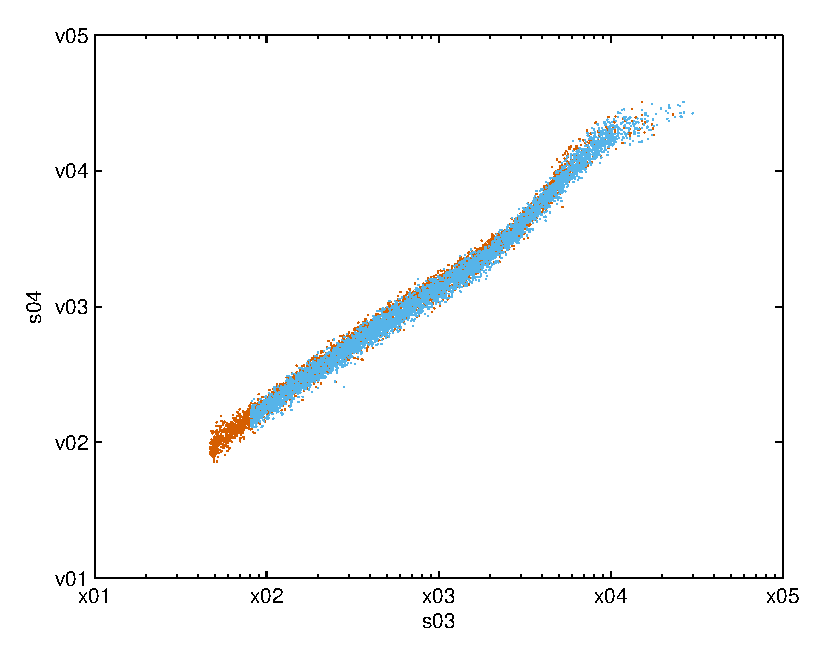
\includegraphics{SNR_scaled.eps}}%
\end{psfrags}%
%
% End SNR_scaled.tex
\end{document}
% See http://www.mathworks.de/matlabcentral/fileexchange/loadFile.do?objectId=4638
% for recent versions of laprint.m.
%
% created by:           LaPrint version 3.16 (13.9.2004)
% created on:           04-Aug-2012 17:56:20
% eps bounding box:     15 cm x 11.25 cm
% comment:              
%
\begin{psfrags}%
\psfragscanon%
%
% text strings:
\psfrag{s03}[t][t]{\color[rgb]{0,0,0}\setlength{\tabcolsep}{0pt}\begin{tabular}{c}{\Large$f_\ast/\mathrm{Hz}$}\end{tabular}}%
\psfrag{s04}[b][b]{\color[rgb]{0,0,0}\setlength{\tabcolsep}{0pt}\begin{tabular}{c}{\Large$\rho_\ast$}\end{tabular}}%
%
% xticklabels:
\psfrag{x01}[t][t]{$10^{-5}$}%
\psfrag{x02}[t][t]{$10^{-4}$}%
\psfrag{x03}[t][t]{$10^{-3}$}%
\psfrag{x04}[t][t]{$10^{-2}$}%
\psfrag{x05}[t][t]{$10^{-1}$}%
%
% yticklabels:
\psfrag{v01}[r][r]{$10^{-2}$}%
\psfrag{v02}[r][r]{$1$}%
\psfrag{v03}[r][r]{$10^{2}$}%
\psfrag{v04}[r][r]{$10^{4}$}%
\psfrag{v05}[r][r]{$10^{6}$}%
%
% Figure:
\resizebox{12cm}{!}{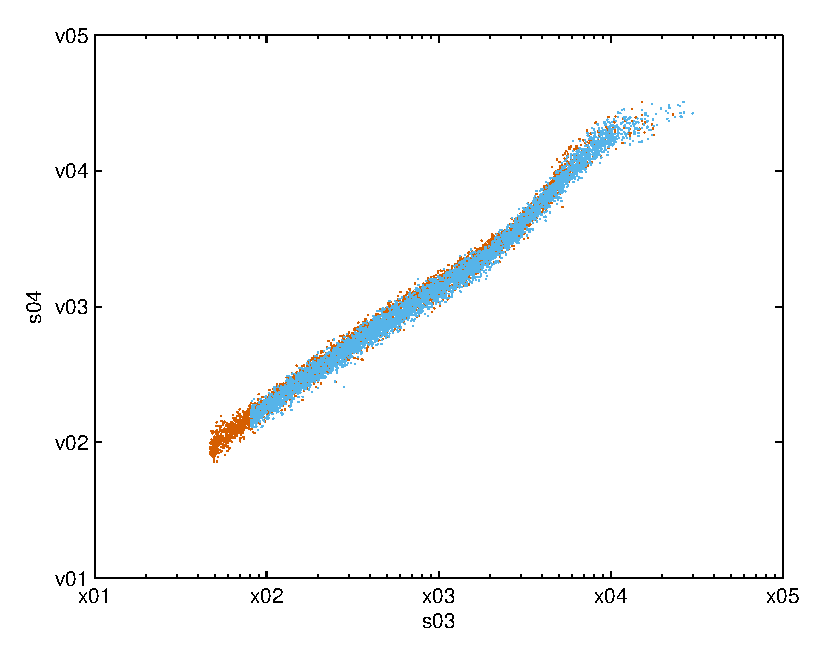
\includegraphics{SNR_scaled.eps}}%
\end{psfrags}%
%
% End SNR_scaled.tex
\end{document}
% See http://www.mathworks.de/matlabcentral/fileexchange/loadFile.do?objectId=4638
% for recent versions of laprint.m.
%
% created by:           LaPrint version 3.16 (13.9.2004)
% created on:           04-Aug-2012 17:56:20
% eps bounding box:     15 cm x 11.25 cm
% comment:              
%
\begin{psfrags}%
\psfragscanon%
%
% text strings:
\psfrag{s03}[t][t]{\color[rgb]{0,0,0}\setlength{\tabcolsep}{0pt}\begin{tabular}{c}{\Large$f_\ast/\mathrm{Hz}$}\end{tabular}}%
\psfrag{s04}[b][b]{\color[rgb]{0,0,0}\setlength{\tabcolsep}{0pt}\begin{tabular}{c}{\Large$\rho_\ast$}\end{tabular}}%
%
% xticklabels:
\psfrag{x01}[t][t]{$10^{-5}$}%
\psfrag{x02}[t][t]{$10^{-4}$}%
\psfrag{x03}[t][t]{$10^{-3}$}%
\psfrag{x04}[t][t]{$10^{-2}$}%
\psfrag{x05}[t][t]{$10^{-1}$}%
%
% yticklabels:
\psfrag{v01}[r][r]{$10^{-2}$}%
\psfrag{v02}[r][r]{$1$}%
\psfrag{v03}[r][r]{$10^{2}$}%
\psfrag{v04}[r][r]{$10^{4}$}%
\psfrag{v05}[r][r]{$10^{6}$}%
%
% Figure:
\resizebox{12cm}{!}{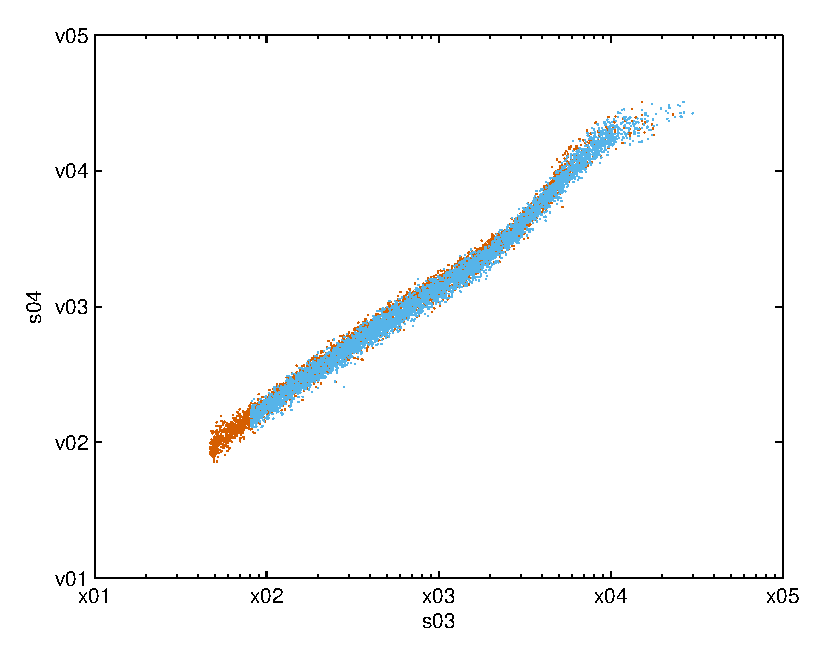
\includegraphics{SNR_scaled.eps}}%
\end{psfrags}%
%
% End SNR_scaled.tex
\end{document}
% See http://www.mathworks.de/matlabcentral/fileexchange/loadFile.do?objectId=4638
% for recent versions of laprint.m.
%
% created by:           LaPrint version 3.16 (13.9.2004)
% created on:           06-Aug-2012 11:26:09
% eps bounding box:     15 cm x 11.25 cm
% comment:              
%
\begin{psfrags}%
\psfragscanon%
%
% text strings:
\psfrag{s05}[t][t]{\color[rgb]{0,0,0}\setlength{\tabcolsep}{0pt}\begin{tabular}{c}{\Large$f_\ast/\mathrm{Hz}$}\end{tabular}}%
\psfrag{s06}[b][b]{\color[rgb]{0,0,0}\setlength{\tabcolsep}{0pt}\begin{tabular}{c}{\Large$\rho_\ast$}\end{tabular}}%
\psfrag{s10}[][]{\color[rgb]{0,0,0}\setlength{\tabcolsep}{0pt}\begin{tabular}{c} \end{tabular}}%
\psfrag{s11}[][]{\color[rgb]{0,0,0}\setlength{\tabcolsep}{0pt}\begin{tabular}{c} \end{tabular}}%
\psfrag{s12}[l][l]{\color[rgb]{0,0,0}M32}%
\psfrag{s13}[l][l]{\color[rgb]{0,0,0}{\large{Galactic centre}}}%
\psfrag{s14}[l][l]{\color[rgb]{0,0,0}{\large{M32}}}%
%
% xticklabels:
\psfrag{x01}[t][t]{$10^{-5}$}%
\psfrag{x02}[t][t]{$10^{-4}$}%
\psfrag{x03}[t][t]{$10^{-3}$}%
\psfrag{x04}[t][t]{$10^{-2}$}%
\psfrag{x05}[t][t]{$10^{-1}$}%
%
% yticklabels:
\psfrag{v01}[r][r]{$10^{-2}$}%
\psfrag{v02}[r][r]{$10^{0}$}%
\psfrag{v03}[r][r]{$10^{2}$}%
\psfrag{v04}[r][r]{$10^{4}$}%
\psfrag{v05}[r][r]{$10^{6}$}%
%
% Figure:
\resizebox{12cm}{!}{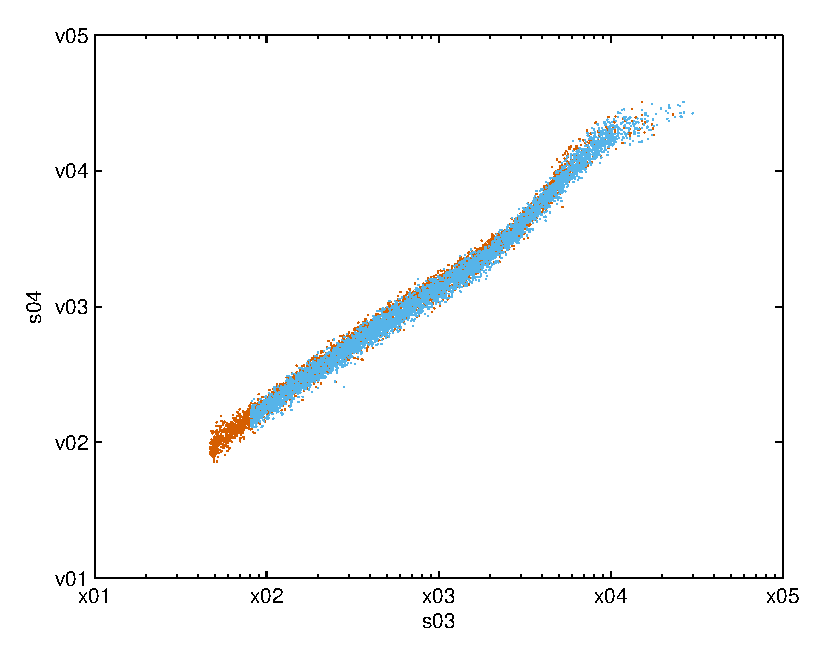
\includegraphics{SNR_scaled.eps}}%
\end{psfrags}%
%
% End SNR_scaled.tex
